\section{チャームバリオン分光実験(J-PARC E50 実験)}
我々は、大強度陽子加速器施設(J-PARC)のハドロン実験施設内にある高運動量ビームラインにおいてチャームバリオン分光実験(J-PARC E50 実験)を計画している。
図\ref{charmed_baryon_generation}にチャームバリオン分光実験におけるチャームバリオン生成反応の模式図を示す。
実験では、$\SI{20}{\GeV / c}$の高運動量2次$\pi^-$ビームを液体水素標的に照射し、生成されたチャームバリオンの励起状態を観測する。
チャームバリオン$(Y_c^{*+})$は$(\ref{charmed_baryon_reaction})$式に示す反応によって生成する。
この時生成される$D^{*-}$は$(\ref{d_reaction})$式に示す崩壊モードにより、2つの$\pi^-$と1つの$K$に崩壊する。
これらの崩壊粒子と入射$\pi^-$ビームの四元運動量を測定することで、missing mass spectroscopyによりチャームバリオンの質量スペクトルを得る。

\begin{equation}
  \label{charmed_baryon_reaction}
  \pi^- + p \rightarrow Y_c^{*+} + D^{*-}
\end{equation}

\begin{equation}
  \label{d_reaction}
  D^{*-} \rightarrow \pi^- + \bar{D}^0 \rightarrow \pi^- + \pi^- + K^+
\end{equation}

\begin{figure}[htbp]
  \label{charmed_baryon_generation}
  \centering
  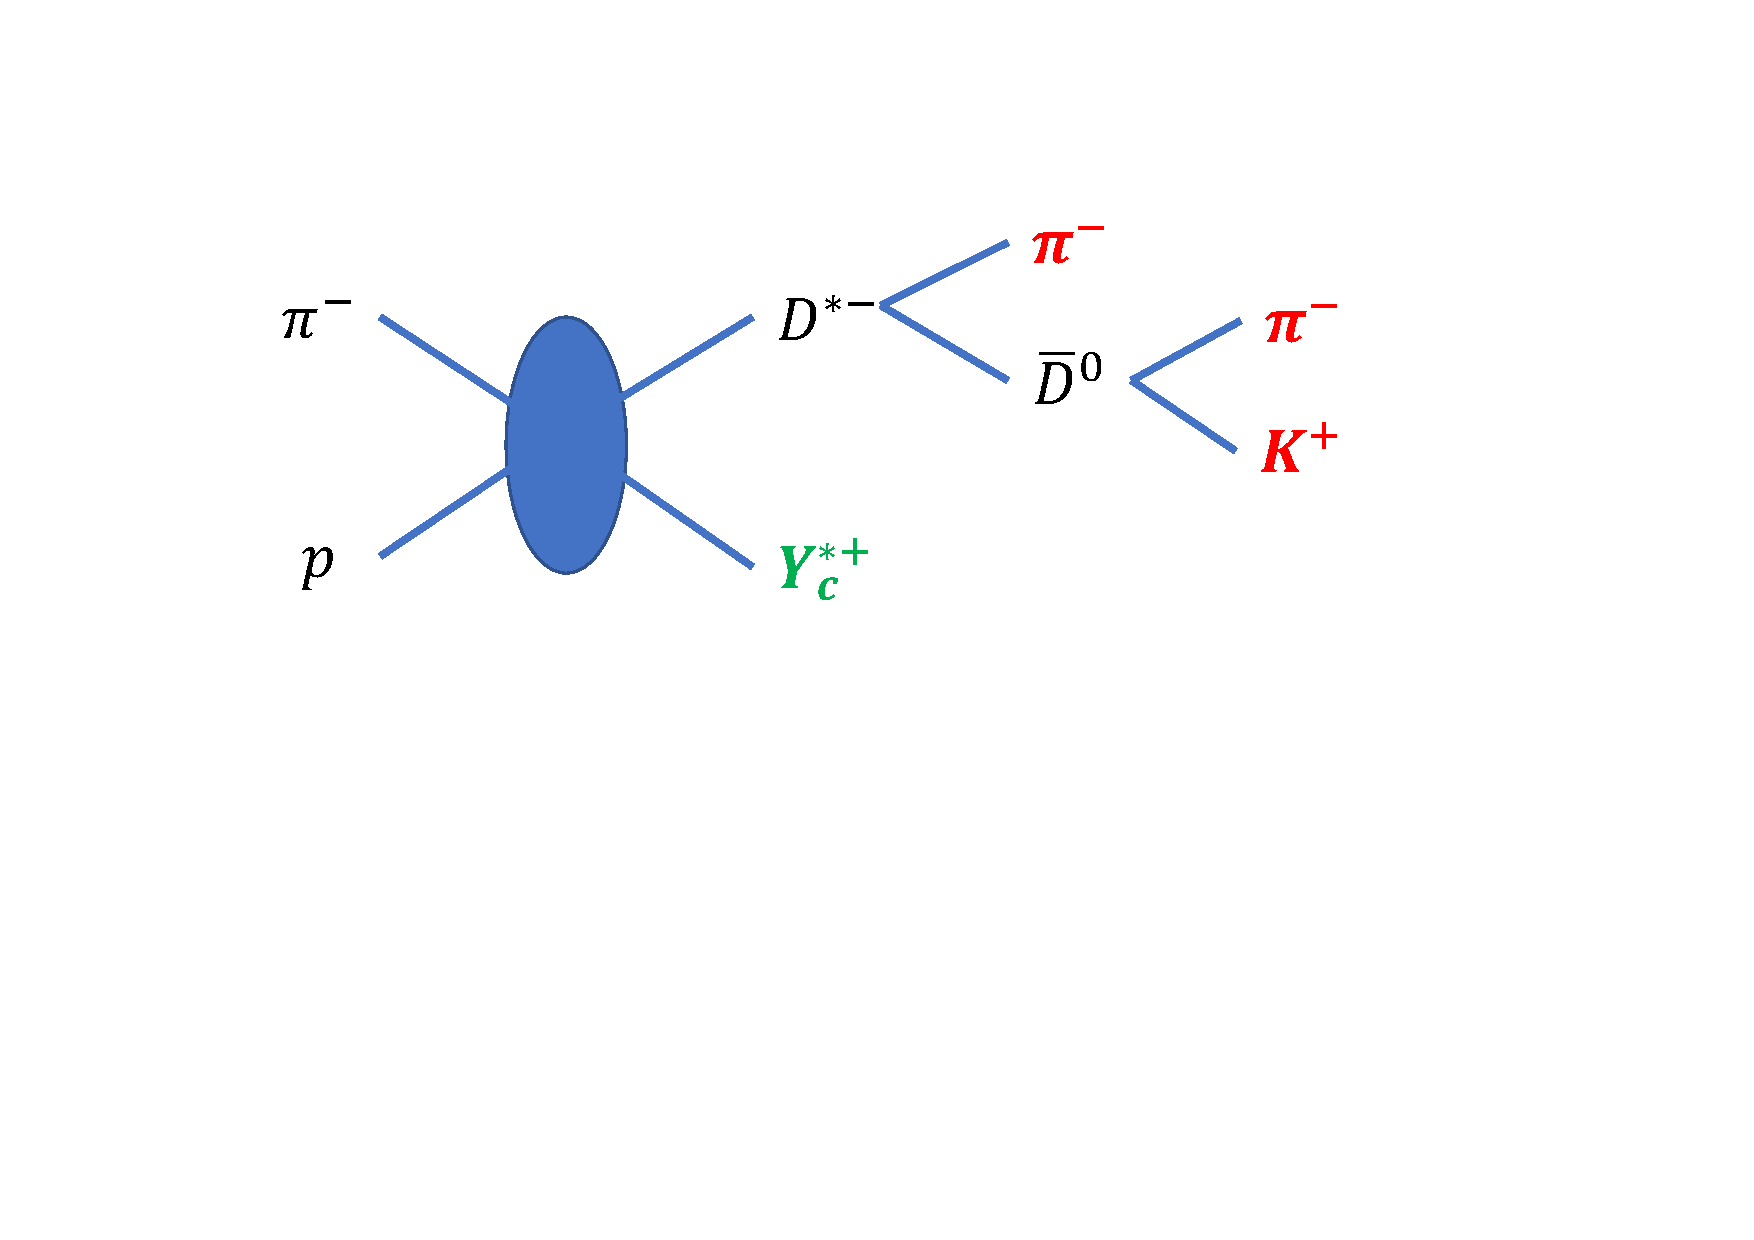
\includegraphics[width=15cm]{images/chapter1/charmed_baryon_generation.pdf}
  \caption{チャームバリオン生成反応の模式図。終状態の$K^+,\pi^-,\pi^-$と入射ビームの四元運動量を測定することで、チャームバリオンの生成を同定しその質量情報を得る。}
\end{figure}